\documentclass[a4paper,12pt]{article}
\usepackage[utf8]{inputenc}
\usepackage{geometry}
\geometry{
 a4paper,
 left=1.25in,
 right=1.25in,
 top=1in,
 }
\usepackage[croatian,english]{babel}    %za hrvatske naslove
\usepackage[nottoc]{tocbibind}  %za pravilan table of content
\usepackage{graphicx}   %za dodavanje slika
\usepackage{amsmath}    %za matematičke forumele
\usepackage{subcaption} %za dvije slike u jednoj
\usepackage{booktabs}   %za bolje tablice

% Zamijenio \usepackage{cite} s natbib
\usepackage[numbers,sort&compress]{natbib}

% Poboljšanja za formatiranje bibliografije
\usepackage{url}
\usepackage{breakurl}
\def\UrlBreaks{\do\/\do-\do_\do.\do=\do?\do&\do:\do\%}
\urlstyle{same}  % Koristi isti font kao ostatak teksta

\usepackage[T1]{fontenc}
\usepackage{xcolor}
\usepackage{minted}
\usepackage{listings}
\lstset{
    inputencoding=utf8,
    extendedchars=true,
    literate={š}{{\v{s}}}1
             {đ}{{\dj}}1
             {č}{{\v{c}}}1
             {ć}{{\v{c}}}1
             {ž}{{\v{z}}}1
             {Š}{{\v{S}}}1
             {Đ}{{\Dj}}1
             {Č}{{\v{C}}}1
             {Ć}{{\v{C}}}1
             {Ž}{{\v{Z}}}1
}
% Definicija za JSON prikaz
\lstdefinelanguage{json}{
    basicstyle=\ttfamily\small,
    numbers=left,
    numberstyle=\tiny\color{gray},
    stepnumber=1,
    numbersep=5pt,
    showstringspaces=false,
    breaklines=true,
    frame=single,
    backgroundcolor=\color{gray!10},
    literate=
     *{0}{{{\color{blue}0}}}{1}
      {1}{{{\color{blue}1}}}{1}
      {2}{{{\color{blue}2}}}{1}
      {3}{{{\color{blue}3}}}{1}
      {4}{{{\color{blue}4}}}{1}
      {5}{{{\color{blue}5}}}{1}
      {6}{{{\color{blue}6}}}{1}
      {7}{{{\color{blue}7}}}{1}
      {8}{{{\color{blue}8}}}{1}
      {9}{{{\color{blue}9}}}{1}
      {:}{{{\color{black}:}}}{1}
      {,}{{{\color{black},}}}{1}
      {"}{{{\color{red}"}}}{1}
}
\begin{document}
\begin{center}
SVEUČILIŠTE JURJA DOBRILE U PULI 

FAKULTET INFORMATIKE

\vspace{45mm} 

\textbf{Petar Prenc}

\vspace{20mm} 

\textbf{Naslov}

\vspace{5mm}
DIPLOMSKI RAD

\vfill

%Upisat tocan mjesec i godinu
Pula, ožujak, 2027. godine
\end{center}

\pagenumbering{gobble}
\clearpage
\newpage
\begin{center}
SVEUČILIŠTE JURJA DOBRILE U PULI 

FAKULTET INFORMATIKE

\vspace{45mm} 

\textbf{Petar Prenc}

\vspace{20mm} 

\textbf{Naslov}

\vspace{5mm}
DIPLOMSKI RAD

\end{center}

\vspace{45mm}

\textbf{JMBAG: 0119034299, redovni student}

\textbf{Studijski smjer: Informatika}
\bigskip

\textbf{Kolegij: ?}

\textbf{Znanstveno područje : Društvene znanosti}

\textbf{Znanstveno polje : Informacijske i komunikacijske znanosti}

\textbf{Znanstvena grana : Informacijski sustavi i informatologija}
\bigskip

\textbf{Mentor: izv. prof. dr. sc. Nikola Tanković}

\vfill

\begin{center}

%Upisat tocan mjesec i godinu
Pula, ožujak, 2027. godine

\end{center}
\pagenumbering{gobble}
\clearpage
\newpage
%Resetirat margine
\restoregeometry
\selectlanguage{croatian}
\begin{abstract}

Sažetak na hrvatskom jeziku.

\end{abstract}
\begin{small}
\textbf{Ključne riječi} : 
\end{small}

\bigskip

\selectlanguage{english}
\begin{abstract}

Abstract in English.

\end{abstract}
\begin{small}
\textbf{Keywords} : 
\end{small}

\pagenumbering{gobble}
\clearpage
\newpage
\selectlanguage{croatian}
\tableofcontents
\pagenumbering{gobble}
\clearpage
\newpage
\pagenumbering{arabic}
\section{Uvod}

Konverzacijska umjetna inteligencija (AI) i chatbotovi postali su neizostavan dio suvremenog digitalnog ekosustava, transformirajući način na koji poduzeća komuniciraju sa svojim korisnicima. Chatbotovi su dizajnirani kao komunikacijski kanali koji omogućuju neprekidnu dostupnost 24 sata dnevno, 7 dana u tjednu, služeći u različite svrhe, od odgovaranja na često postavljana pitanja do angažiranja korisnika i prikupljanja dubljih uvida u njihove potrebe. Ovi sustavi nastoje oponašati ljudsku interakciju, omogućujući duže i često nestrukturirane razgovore, što ih razlikuje od tradicionalnih sustava za dijalog orijentiranih na zadatke koji se oslanjaju na unaprijed definirane "okvire" ili "slotove" za prikupljanje informacija. Moderni sustavi često kombiniraju aspekte oba pristupa, spajajući fluidnost otvorenog chata sa strukturiranom, ciljanom prirodom dijaloga orijentiranog na zadatke.

Značajan napredak u računalnoj snazi, dostupnost ogromnih skupova podataka i razvoj sofisticiranih modela strojnog učenja doveli su do značajnog poboljšanja sustava za razumijevanje i generiranje prirodnog jezika. Ti su napreci omogućili stvaranje konverzacijskih AI sustava koji mogu generirati odgovore riječ po riječ ili dohvaćati najprikladnije odgovore iz skupa unaprijed definiranih kandidata.

Sveučilišta diljem svijeta suočavaju se s izazovima u pružanju brze i točne podrške studentima, posebno tijekom procesa upisa i tijekom studija. Studenti često postavljaju pitanja o uvjetima upisa, rasporedima predavanja, ispitnim rokovima, stipendijama i drugim administrativnim procesima. Tradicionalni kanali podrške, poput e-pošte, telefonskih poziva ili osobnih konzultacija, često su preopterećeni, što dovodi do kašnjenja i frustracija kod studenata. Osim toga, statične FAQ stranice na web stranicama fakulteta ne mogu uvijek odgovoriti na raznolike oblike pitanja koje studenti postavljaju, posebno ako su formulirana na različite načine.

Chatbotovi temeljeni na umjetnoj inteligenciji nude rješenje za ove izazove, omogućujući automatizaciju odgovora na česta pitanja i pružanje trenutne podrške. Projekt Sembot razvijen je s ciljem stvaranja jednostavnog, skalabilnog i lako prilagodljivog chatbota koji koristi moderne tehnologije za obradu prirodnog jezika. Koristeći Semantic Router i FastAPI, Sembot može razumjeti semantički slične upite i pružiti točne odgovore, dok jednostavno web sučelje omogućuje studentima intuitivnu interakciju.

Ovaj rad pruža sveobuhvatan pregled projekta, uključujući tehničku arhitekturu, implementaciju semantičkog usmjeravanja, upravljanje podacima, prijedloge za sustav preporuke te potencijalne buduće nadogradnje. Također se razmatraju alternative trenutnom pristupu i potencijalni izazovi u implementaciji.
\newpage
\section{Pregled literature}

\subsection{Pregled Arhitekture}
Implementacija chatbot sustava za studentska pitanja temelji se na modularnoj arhitekturi koja omogućava skalabilnost i održivost. Sustav je dizajniran kao mikroservisna aplikacija koja integrira semantic routing kao osnovni mehanizam za usmjeravanje korisničkih upita prema relevantnim odgovorima.
Arhitektura sustava sastoji se od pet glavnih komponenti: korisničko sučelje (frontend), API gateway, semantic routing engine, baza znanja i recommendation servis. Svaka komponenta ima jasno definirane odgovornosti i komunicira s ostalima kroz standardizirane API-je.

\subsection{Tehnološki Stack}
Odabir tehnologija temeljio se na potrebi za visokom performansom, skalabilnošću i jednostavnošću održavanja. Backend je implementiran u Python programskom jeziku koristeći FastAPI framework zbog njegove brzine i automatske dokumentacije API-ja.
Za embedding modele korišten je sentence-transformers s pretreniranim modelom 'all-MiniLM-L6-v2' koji pruža dobar balans između kvalitete vektora i brzine izvršavanja. Vector store implementiran je pomoću FAISS biblioteke koja omogućava brzo pretraživanje najbližih susjeda u višedimenzionalnom prostoru.

\subsection{Motivacija}

Motivacija za razvoj Sembota proizlazi iz potrebe za automatizacijom podrške studentima, posebno u kontekstu sveučilišta s velikim brojem upita. Projekt ima za cilj smanjiti opterećenje na administrativno osoblje, omogućiti studentima brži pristup informacijama i stvoriti platformu koja se može lako prilagoditi različitim fakultetima i obrazovnim institucijama.

\subsection{Ciljevi projekta}

\begin{enumerate}
    \item Razviti chatbot koji može odgovarati na česta pitanja studenata koristeći semantičko pretraživanje.
    \item Omogućiti jednostavno proširenje sustava dodavanjem novih pitanja i odgovora.
    \item Osigurati skalabilnost i fleksibilnost sustava za buduće nadogradnje.
    \item Pružiti intuitivno korisničko sučelje dostupno putem web preglednika.
\end{enumerate}

\subsection{Problem}
Studenti se suočavaju s brojnim izazovima prilikom traženja informacija o fakultetskim procesima. Na primjer, pitanja poput "Koji su uvjeti za upis?" ili "Kada počinju predavanja?" često zahtijevaju trenutne odgovore, ali administrativni uredi nemaju dovoljno resursa za obradu velikog broja upita. Osim toga, postojeći sustavi, poput FAQ stranica, često su ograničeni na unaprijed definirane odgovore i ne mogu obraditi varijacije u formulaciji pitanja. Ovo dovodi do neefikasnosti, povećanog opterećenja na osoblje i lošijeg korisničkog iskustva.

Ključni izazovi:
\begin{enumerate}
    \item Veliki broj upita: Sveučilišta dobivaju stotine ili tisuće upita dnevno tijekom upisnih rokova.
    \item Raznolikost formulacija: Studenti postavljaju ista pitanja na različite načine, što otežava automatsku obradu.
    \item Ograničeni resursi: Administrativno osoblje ne može uvijek pružiti trenutne odgovore.
    \item Skalabilnost: Postojeći sustavi često nisu prilagođeni za obradu velikih količina podataka ili novih vrsta upita.
\end{enumerate}

\subsection{Alternativna rješenja}

Postoji nekoliko pristupa za rješavanje ovog problema, svaki s prednostima i nedostacima:

\begin{enumerate}
   \item \textbf{Statične FAQ stranice}:
   \begin{itemize}
       \item \textbf{Opis}: Web stranice s unaprijed definiranim pitanjima i odgovorima.
       \item \textbf{Prednosti}: Jednostavne za implementaciju, ne zahtijevaju složene tehnologije.
       \item \textbf{Nedostaci}: Ne mogu obraditi varijacije u formulaciji pitanja, nisu interaktivne, teško se skaliraju za veliki broj pitanja.
       \item \textbf{Primjena}: Pogodne za male institucije s ograničenim brojem upita.
   \end{itemize}
   
   \item \textbf{E-mail ili telefonska podrška}:
   \begin{itemize}
       \item \textbf{Opis}: Studenti kontaktiraju administrativno osoblje putem e-pošte ili telefona.
       \item \textbf{Prednosti}: Omogućuje personalizirane odgovore, pogodno za složene upite.
       \item \textbf{Nedostaci}: Vremenski zahtjevno, ne skalira se dobro s velikim brojem upita, skupo za održavanje.
       \item \textbf{Primjena}: Prikladno za specifične, rijetke upite koji zahtijevaju ljudsku intervenciju.
   \end{itemize}
   
   \item \textbf{Chatbotovi temeljeni na ključnim riječima}:
   \begin{itemize}
       \item \textbf{Opis}: Sustavi koji traže podudarnosti ključnih riječi između upita i baze podataka.
       \item \textbf{Prednosti}: Relativno jednostavni za implementaciju, brzi za male baze podataka.
       \item \textbf{Nedostaci}: Ne razumiju kontekst ili semantičku sličnost, što dovodi do netočnih odgovora za varijacije pitanja.
       \item \textbf{Primjena}: Pogodni za jednostavne sustave s ograničenim brojem pitanja.
   \end{itemize}
   
   \item \textbf{AI chatbotovi s prirodnim jezikom}:
   \begin{itemize}
       \item \textbf{Opis}: Chatbotovi temeljeni na naprednim modelima poput BERT-a, GPT-a ili sličnih.
       \item \textbf{Prednosti}: Razumiju prirodni jezik, mogu obraditi složene upite, prilagodljivi su.
       \item \textbf{Nedostaci}: Zahtijevaju značajne računalne resurse, složeni su za implementaciju, često zahtijevaju plaćene API-je.
       \item \textbf{Primjena}: Idealni za velike institucije s velikim brojem upita i dostupnim resursima.
   \end{itemize}
\end{enumerate}

Sembot kombinira prednosti AI chatbotova s jednostavnošću i skalabilnošću, koristeći Semantic Router za razumijevanje prirodnog jezika i FastAPI za efikasnu obradu upita. Ovaj pristup omogućuje fleksibilnost i lako proširenje sustava uz minimalne resurse.



\newpage
\section{Implementacija}

\subsection{Arhitektura projekta}
Projekt Sembot sastoji se od dva glavna dijela: backend i frontend. Backend je izgrađen koristeći FastAPI, Python framework koji omogućuje brzu izradu API-ja s visokim performansama. Semantic Router koristi OpenAI-jeve embeddinge za pretvaranje upita i pitanja u vektorske reprezentacije, omogućujući semantičko pretraživanje. Podaci se pohranjuju u JSON datoteku (qa\_data.json), koja služi kao jednostavna baza podataka. Frontend je implementiran kao web aplikacija koristeći HTML, CSS i JavaScript, pružajući korisnicima jednostavno sučelje za interakciju s chatbotom.

\begin{figure}
    \centering
    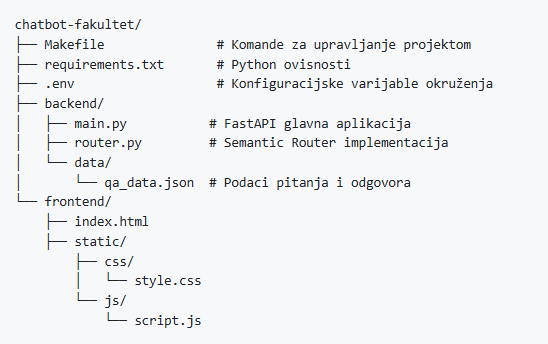
\includegraphics[width=1\linewidth]{hijerarhija.png}
    \caption{Struktura projekta}
    \label{fig:enter-label}
\end{figure}

\subsection{Prednosti arhitekture}

\begin{enumerate}
    \item Modularnost: Backend i frontend su odvojeni, što olakšava održavanje i nadogradnju.
    \item Skalabilnost: FastAPI omogućuje brzu obradu velikog broja upita.
    \item Proširivost: Novi parovi pitanje-odgovor mogu se dodati u JSON datoteku bez promjene koda.
\end{enumerate}

\begin{figure}
    \centering
    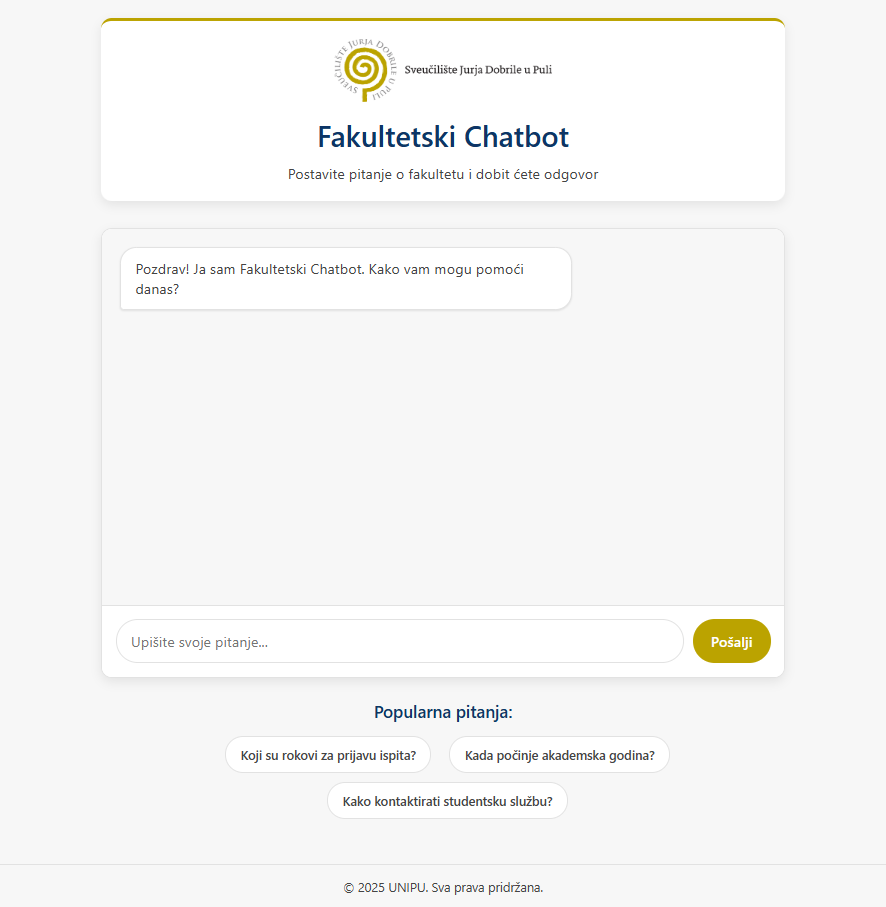
\includegraphics[width=1\linewidth]{sembot_1.png}
    \caption{Početno sučelje aplikacije}
    \label{fig:enter-label}
\end{figure}

\begin{figure}
    \centering
    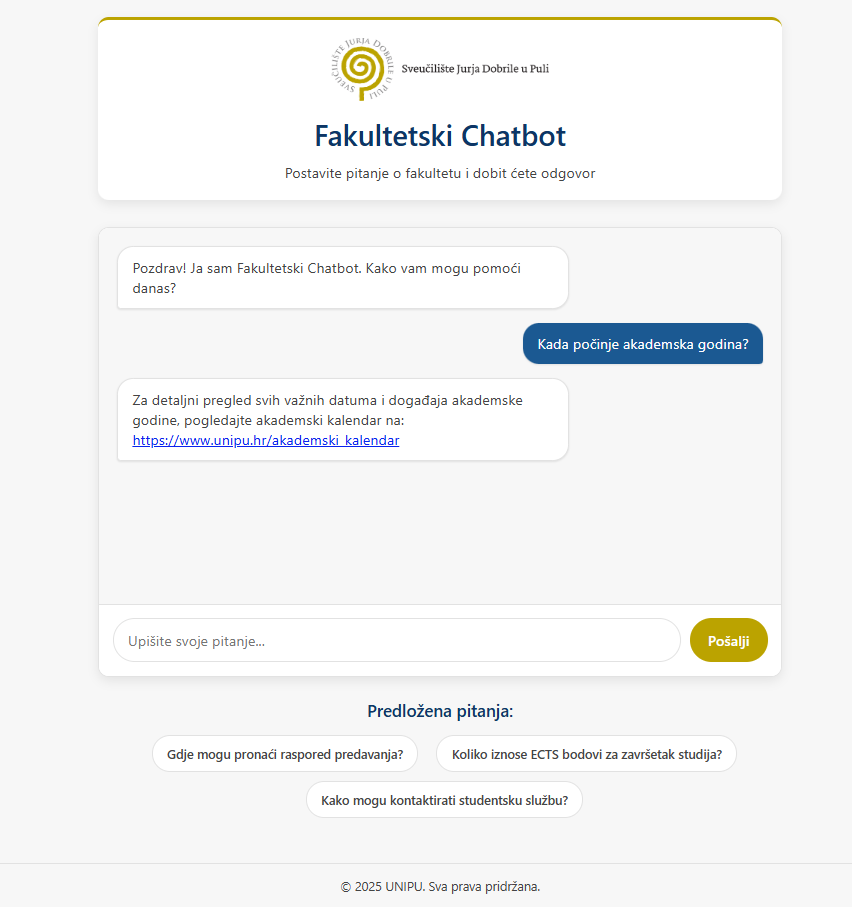
\includegraphics[width=1\linewidth]{sembot_2.png}
    \caption{Odgovor na pitanje s url linkom}
    \label{fig:enter-label}
\end{figure}

\begin{figure}
    \centering
    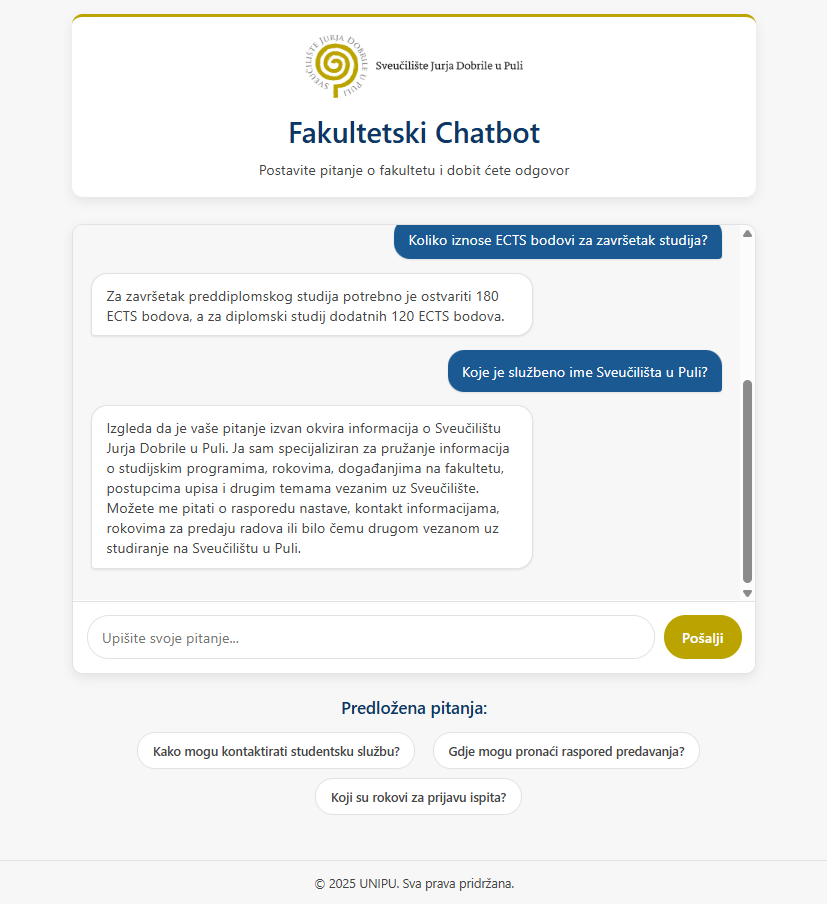
\includegraphics[width=1\linewidth]{sembot_3.png}
    \caption{Odgovor na pitanje bez url linka}
    \label{fig:enter-label}
\end{figure}

\begin{figure}
    \centering
    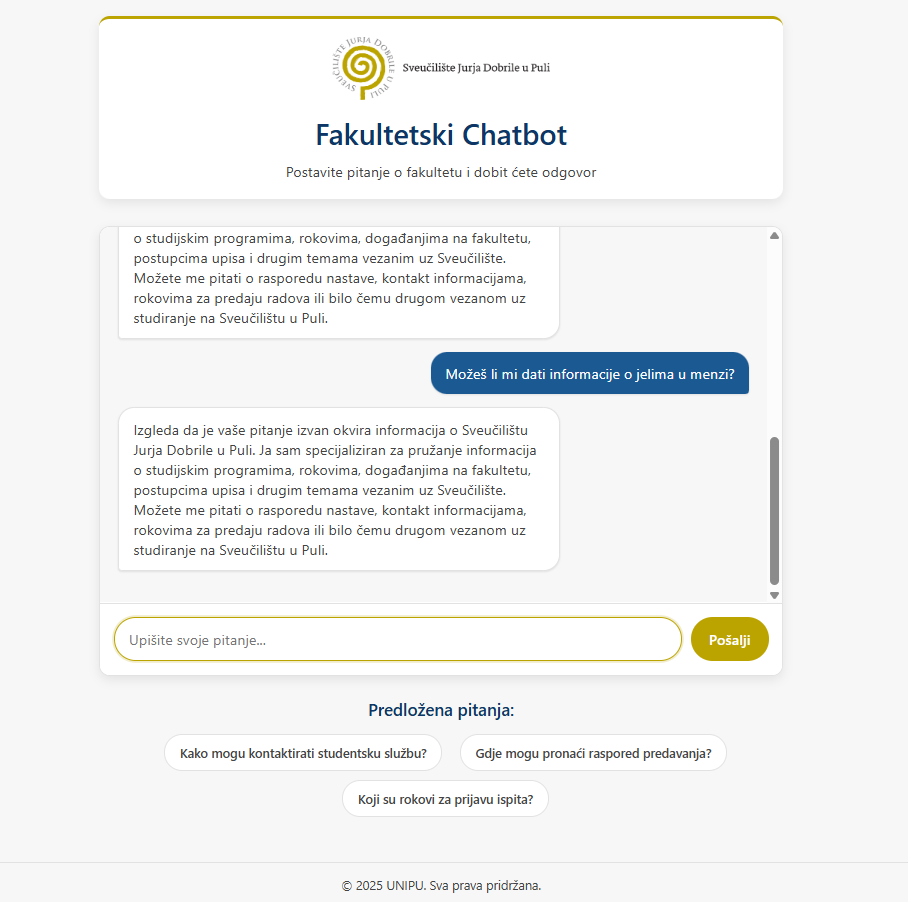
\includegraphics[width=1\linewidth]{sembot_4.png}
    \caption{Prikaz default odgovora}
    \label{fig:enter-label}
\end{figure}
\newpage
\section{Semantic routing}
\subsection{Općenito o Semantic Routingu}

Semantičko usmjeravanje (SR) je pristup planiranju ruta temeljen na učenju, koji obrađuje bogate korisničke upite koji specificiraju različite kriterije i preferencije, nadilazeći ograničenja klasičnih algoritama planiranja ruta. Ono predstavlja kontekstualnu i višeobjektivnu generalizaciju tradicionalnog planiranja ruta. U kontekstu konverzacijske umjetne inteligencije, SR funkcionira kao iznimno brz sloj za donošenje odluka za LLM-ove i AI agente, usmjeravajući zahtjeve na temelju semantičkog značenja, umjesto da se oslanja na spore LLM generacije ili krute sustave temeljene na pravilima.

Temeljni princip semantičkog usmjeravanja je razumijevanje namjere i značenja korisničkog upita. To se postiže pretvaranjem upita u numeričke reprezentacije, poznate kao vektorski ugradci (eng. vector embeddings), koji hvataju semantičko značenje. Značenje se geometrijski prikazuje u visokodimenzionalnom "semantičkom prostoru", gdje su semantički slične točke podataka (upiti, dokumenti, rute) pozicionirane bliže jedna drugoj. Odluke o usmjeravanju donose se usporedbom ugradnje novog zahtjeva s ugradnjama unaprijed definiranih "ruta" ili "namjera". Najbliže podudaranje određuje odgovarajuću akciju ili odgovor. Ovaj pristup omogućuje stvaranje modularnih RAG aplikacija usmjeravanjem upita na različite cjevovode (npr. specifične LLM-ove, vanjske alate, česta pitanja). To pruža granularnu kontrolu nad rukovanjem upitima i pomaže u izbjegavanju odgovora izvan predviđenog opsega.

\subsection{Matematika iza Semantic Routinga}
Proces semantičkog usmjeravanja započinje transformacijom sirovog ulaznog sadržaja – bilo teksta, slika ili zvuka – u numeričke reprezentacije poznate kao vektorski ugradci. Ovi su ugradci pažljivo izrađeni kako bi uhvatili inherentno semantičko značenje podataka. Zatim se pozicioniraju unutar visokodimenzionalnog "semantičkog prostora", matematičke konstrukcije gdje su točke podataka sa sličnim značenjima geometrijski smještene u neposrednoj blizini. Na primjer, ugradci za "automobil" i "vozilo" bili bi blizu, dok bi "automobil" i "banana" bili udaljeni. Proces konverzije obavljaju specijalizirani modeli neuronskih mreža nazvani **enkoderi** (također poznati kao bi-enkoderi ili modeli ugradnje). Ovi modeli analiziraju značajke i semantička svojstva ulaznog sadržaja i izlaze fiksni vektor, obično sastavljen od stotina ili tisuća brojeva s pomičnim zarezom. Istaknuti primjeri tekstualnih enkodera uključuju Word2Vec, BERT, Sentence-BERT i Universal Sentence Encoder. Za multimodalne ulaze, enkoderi poput CLIPEncoder-a ili VitEncoder-a mogu smjestiti slike u isti semantički prostor kao i tekst, omogućujući usporedbe između različitih modaliteta.
Nakon što su upiti i unaprijed definirane rute (ili njihovi povezani iskazi/reference) pretvoreni u vektore, njihova se semantička sličnost kvantitativno izračunava. **Kosinusna sličnost** je široko prihvaćena matematička mjera koja kvantificira sličnost između dviju vektora izračunavanjem kosinusa kuta između njih. Rezultirajuća vrijednost kreće se od -1 (što ukazuje na potpuno suprotne smjerove, odnosno savršenu nepodobnost) do 1 (što ukazuje na identične smjerove, odnosno savršenu sličnost), pri čemu 0 predstavlja ortogonalnost (bez sličnosti). U praktičnim primjenama, često se koristi s normaliziranim vektorima, gdje ishod ovisi isključivo o smjeru vektora, a ne o njihovoj veličini. Matematička formula za kosinusnu sličnost za dva vektora $A$ i $B$ definirana je kao:

$$CosineSimilarity(A, B) = \frac{A \cdot B}{||A|| \times ||B||}$$

Gdje je $A \cdot B$ skalarni produkt vektora A i B, a $||A||$ i $||B||$ označavaju euklidske norme (veličine) vektora A i B. Osim kosinusne sličnosti, za izračun sličnosti koriste se i druge matematičke operacije poput euklidske udaljenosti i skalarnog produkta. Kosinusna sličnost je posebno učinkovita kada su vektori unaprijed normalizirani, jer se izračun pojednostavljuje na izravan skalarni produkt.

Sustavi semantičkog usmjeravanja, poput SemanticRoutera tvrtke RedisVL, implementiraju klasifikacijski pristup tipa K-najbližih susjeda (KNN) za donošenje odluka. Sustav radi s unaprijed definiranim objektima `Route`, od kojih svaki sadrži skup `referenci` (primjera iskaza) koji zajedno definiraju semantički opseg ili "površinu" te određene rute. Kada se primi novi korisnički zahtjev, izračunava se njegov vektorski ugradak i zatim se uspoređuje s ugradcima svih unaprijed definiranih referenci rute. Ključni element u ovom procesu donošenja odluka je `prag udaljenosti` (eng. `distance\_threshold`). Svakoj ruti dodjeljuje se jedinstveni `prag udaljenosti` (ili prag sličnosti). Da bi se upit uspješno usmjerio na određenu rutu, semantička udaljenost između ugradka upita i barem jedne reference te rute mora biti manja ili jednaka ovom unaprijed definiranom pragu.[13] Ako se ne pronađe podudaranje unutar praga bilo koje rute (tj. upit nije semantički dovoljno blizu nijednoj ruti), sustav bilježi "promašaj", što ukazuje da nije pronađena prikladna ruta.

\subsection{Prednosti i izazovi}
\paragraph{Prednosti}
\begin{itemize}
    \item Razumijevanje konteksta i varijacija u jeziku.
    \item Visoka točnost u pronalaženju relevantnih odgovora.
    \item Fleksibilnost za različite domene i jezike.
\end{itemize}

\paragraph{Izazovi}
\begin{itemize}
    \item Zahtijeva računalne resurse za generiranje embeddinga.
    \item Ovisnost o vanjskim API-jima (npr. OpenAI).
    \item Potrebna je dobra kvaliteta podataka u bazi za točne rezultate.
\end{itemize}

\subsection{Primjena u projektu}
U Sembotu, Semantic Router koristi OpenAI-jeve embeddinge za generiranje vektorskih reprezentacija korisničkih upita i pitanja iz qa\_data.json. Proces obrade upita sastoji se od sljedećih koraka:
\begin{itemize}
\item \textbf{Unos upita:} Korisnik unosi pitanje putem web sučelja (npr. "Koji su uvjeti za upis?").
\item \textbf{Pretvorba u vektor:} Upit se šalje na OpenAI API, koji vraća vektorsku reprezentaciju ($v_q$).
\item \textbf{Usporedba s bazom:} Vektor $v_q$ uspoređuje se s vektorima svih pitanja $v_{p_i}$ u bazi podataka koristeći kosinusnu sličnost. U ovom koraku, sustav provjerava je li semantička udaljenost između $v_q$ i barem jedne reference rute manja ili jednaka unaprijed definiranom `pragu udaljenosti` za tu rutu.
\item \textbf{Odabir odgovora:} Pitanje s najvećom kosinusnom sličnošću koje zadovoljava prag udaljenosti odabire se, a povezani odgovor vraća korisniku. Ako se ne pronađe podudaranje unutar praga bilo koje rute, sustav bilježi "promašaj", što ukazuje da nije pronađena prikladna ruta.
\end{itemize}
Proces Semantic Routinga može se vizualizirati kao sljedeći dijagram:
Korisnički upit -> Pretvorba u vektor -> Usporedba s bazom (uz provjeru praga udaljenosti) -> Odabir odgovora -> Prikaz korisniku
\newpage
\section{Sustav preporuke sljedećeg pitanja}
U sustavima dijaloga, problem preporuke sljedećeg pitanja (ili rangiranja sljedećeg iskaza) definira se kao zadatak odabira najprikladnijeg sljedećeg iskaza $u_{n+1}$ (odgovora) iz unaprijed definiranog skupa od $m$ kandidatskih iskaza $\{r_1, r_2,..., r_m\}$, s obzirom na kontekst razgovora $C = \{u_1, u_2,..., u_n\}$ (slijed od $n$ iskaza). Cilj je rangirati ove kandidatske odgovore na temelju njihove prikladnosti za kontekst razgovora, pri čemu se bira onaj s najvišim rezultatom.

Ovaj zadatak predstavlja nekoliko značajnih izazova:
\begin{itemize}
\item \textbf{Implicitna zajednička informacija:} Često postoji implicitna zajednička informacija između konteksta i odgovora koja nije eksplicitno navedena.
\item \textbf{Identificiranje važnih informacija:} Identificiranje važnih informacija (riječi, fraza i rečenica) unutar konteksta i njihovo učinkovito podudaranje s odgovarajućim informacijama u odgovoru je složeno.
\item \textbf{Modeliranje odnosa između višestrukih iskaza:} Modeliranje odnosa između višestrukih iskaza koji čine povijest razgovora također je značajan izazov. Iako neki pristupi pojednostavljuju razgovor na samo posljednji iskaz, uzimanje u obzir **cjelokupnog konteksta** je ključno za bolju izvedbu.
\item \textbf{Ograničeno razumijevanje jezika:} Chatbotovi se suočavaju s poteškoćama u razumijevanju nijansi poput idioma, sarkazma ili igre riječi, što rezultira pogrešnim tumačenjima i irelevantnim odgovorima. Čak i napredni NLP modeli mogu pogrešno protumačiti polisemne pojmove ili regionalne dijalekte.
\item \textbf{Nemogućnost učenja iz iskustva:} Tradicionalni chatbotovi ne mogu prilagoditi odgovore na temelju povijesti razgovora niti poboljšati performanse tijekom vremena.
\item \textbf{Nedostatak emocionalne inteligencije:} Chatbotovi ne mogu prepoznati korisnikovo emocionalno stanje, što može dovesti do neprikladnih ili neosjetljivih odgovora.
\item \textbf{Problem hladnog starta:} Nedostatak visokokvalitetnih povijesnih podataka za nove domene dovodi do loše klasifikacije namjera i irelevantnih putanja ispitivanja.
\item \textbf{Pristranost uzorka u obrascima odgovora:} Chatbotovi mogu angažirati samo digitalno pismene korisnike, iskrivljujući podatke i uvodeći demografsku/bihevioralnu pristranost.
\item \textbf{Slaba dugoročna memorija u LLM-ovima:} LLM-ovi koji pokreću chatbotove često pokazuju slabo dugoročno pamćenje, zaboravljajući ranije unose ili proturječeći sami sebi tijekom razgovora.
\item \textbf{Rukovanje neviđenim scenarijima:} Chatbotovi se često susreću s nepredviđenim scenarijima, što može dovesti do "halucinacija" - generiranja netočnih informacija s visokim stupnjem samopouzdanja.
\end{itemize}


\subsection{Temeljni Principi i metodologije}
Temeljni principi rangiranja sljedećeg pitanja uključuju sofisticirane metode reprezentacije teksta, arhitekture kodiranja i matematičke operacije za izračun sličnosti.

\textbf{Reprezentacija Teksta (Vektorski Ugradci):} Ulazni tekst, uključujući kontekst razgovora i kandidatski odgovor, prvo se pretvara u vektorske ugradke. To su numeričke vektorske reprezentacije riječi, gdje riječi sa sličnim značenjima imaju slične vektorske reprezentacije. Ovi ugradci se često inicijaliziraju unaprijed obučenim modelima poput GloVe-a ili se generiraju modelima kao što su Word2Vec, BERT, Sentence-BERT i Universal Sentence Encoder.

\textbf{Arhitekture Kodiranja (npr. LSTM Dual Enkoderi, Pažljivi Dual Enkoderi):}
\begin{itemize}
\item \textbf{Dual Enkoder Model:} Sastoji se od dva odvojena enkodera (npr. Long Short-Term Memory, LSTM, mreže) koji neovisno izvlače značajke za dijalog kontekst i kandidatski odgovor. Ovi enkoderi transformiraju ulazni tekst varijabilne veličine (sekvencu vektorskih ugradaka riječi) u vektore fiksne duljine, označene kao $C'$ za kontekst i $R'$ za odgovor. Skriveni sloj LSTM enkodera ažurira se svaki put kada se obradi vektorski ugradak riječi.

\item \textbf{Pažljivi Dual Enkoder Model:} Predstavlja napredak u odnosu na standardne dual enkodere, uključujući mehanizam pažnje povrh izvučenih značajki na razini riječi iz oba enkodera. Ovaj mehanizam uči vezu između dijalog konteksta i odgovora na razini riječi. Matrica sličnosti $S$ (npr. koristeći kosinusnu sličnost) definira se na kodiranim značajkama $h_x$ (kontekst) i $h_y$ (odgovor) za mjerenje parnih odnosa riječi.[19] Težine pažnje se izračunavaju (npr. korištenjem softmax funkcije preko eksponencijala unosa matrice sličnosti) i zatim ponderiraju izvorne kodirane značajke prema njihovoj važnosti.
\end{itemize}



\subsection{Matematička osnova izračuna sličnosti}
\subsubsection{Vektorski produkt (u nekim dual enkoderima)}
U nekim poboljšanim arhitekturama LSTM dual enkodera, sličnost između kodiranog kontekstualnog vektora $C'$ i kodiranog vektora odgovora $R'$ izračunava se kao križni produkt $P$. Matematički, ako je $C' = [c_1, c_2,..., c_h]$ i $R' = [r_1, r_2,..., r_h]$ (gdje je $h$ veličina skrivenog sloja), tada je $$P = C' \times R' = [c_1 \cdot r_1, c_2 \cdot r_2,..., c_h \cdot r_h]$$ (element-po-element množenje, često se naziva Hadamardovim produktom u ovom kontekstu). Cilj ovog produkta je uhvatiti zajedničke semantičke i sintaktičke značajke.

\subsubsection{Skalarni produkt (u attentive dual encoderima)}
Konačni rezultat predviđanja za par dijalog kontekst-odgovor u attentive dual enkoderima izračunava se kao skalarni produkt pažljivo ponderiranih značajki konteksta i odgovora: $$score(x, y) = dot((a_x)|h_x, (a_y)|h_y).$$

\subsubsection{Generiranje vjerojatnosnog rezultata} Vektorski rezultat sličnosti (npr. $P$ iz križnog produkta) ili rezultat (iz skalarnog produkta) prosljeđuje se u potpuno povezani sloj. Na izlaz ovog sloja primjenjuje se sigmoidna aktivacijska funkcija, $\sigma(x) = \frac{1}{1 + e^{-x}}$, kako bi se dobio vjerojatnosni rezultat između 0 i 1. Ovaj rezultat ukazuje na vjerojatnost da je kandidatski iskaz ispravan sljedeći iskaz za zadani kontekst i koristi se za rangiranje.

\subsection{Poboljšanje interpretativnosti (attentive dual enkoderi)}
\textbf{Problem:} Standardni mehanizmi pažnje mogu istaknuti nevažne riječi, zamagljujući interpretativnost i potencijalno narušavajući performanse. Enkoderi također mogu izgubiti fine-zrnate informacije na razini riječi.

\begin{itemize}
\item Rješenje 1: \textbf{Regularizacija bez pažnje (minimizacija uzajamne informacije):} Predlaže se novi gubitak regularizacije koji minimizira uzajamnu informaciju između nevažnih riječi konteksta ($h_x$) i značajki odgovora ($h_y$). To prisiljava model da de-naglaava nevane rijei dok naglaava vane.

\item Rješenje 2: \textbf{Rezidualni sloj s sirovim vektorskim ugradcima riječi:} Dodaje se rezidualni sloj koji izravno povezuje sirove vektorske ugradke riječi ($e_x$) s konačnom kodiranom značajkom konteksta, čime se čuva interpretativnost na razini riječi.
\end{itemize}


\subsection{Ukupni Cilj Treninga (attentive dual enkoderi)} Ukupni cilj treninga je min-max igra koja kombinira gubitak dohvaćanja ($L_{ret}$) za maksimiziranje rezultata ispravnih parova dijalog kontekst-odgovor i regularizacijski član uzajamne informacije ($L_{reg}$) za isticanje korisnih informacija: $$\min_{\theta_x,\theta_y} \max_{\theta_D} L_{ret}(\theta_x, \theta_y) + \beta L_{reg}(\theta_x, \theta_y, \theta_D).$$


Sustav preporuke može koristiti istu tehniku semantičke sličnosti kao i Semantic Router. 
Algoritam radi kako slijedi:
\begin{itemize}
    \item Nakon što korisnik postavi upit i dobije odgovor, sustav generira vektorsku reprezentaciju upita ($v_q$).
    \item Uspoređuje ($v_q$) s vektorima svih pitanja ($v_{p_i}$) u bazi podataka.
    \item Odabire $k$ pitanja (npr. $k = 3$) s najvećom kosinusnom sličnošću, isključujući trenutno pitanje.
    \item Prikazuje preporučena pitanja korisniku u sučelju.
\end{itemize}

Ako korisnik pita "Koji su uvjeti za upis?", sustav može predložiti pitanja poput:
\begin{itemize}
\item   "Kako se prijaviti za stipendiju?"
\item   "Kada su rokovi za upis?"
\item   "Koje dokumente treba dostaviti za upis?"
\end{itemize}



\subsection{Buduće nadogradnje}

\begin{itemize}
    \item \textbf{Personalizacija:} Sustav može pratiti povijest korisnikovih upita i prilagođavati preporuke na temelju njihovih interesa.
    \item \textbf{Kontekstualna analiza:} Umjesto samo semantičke sličnosti, sustav može koristiti dodatne informacije, poput kategorija pitanja (npr. upis, stipendije, ispiti).
    \item \textbf{Interaktivni prijedlozi:} Omogućiti korisnicima ocjenjivanje preporuka kako bi se poboljšao algoritam.
\end{itemize}

\newpage
\section{Baza podataka}
Sembot trenutno koristi JSON datoteku (qa\_data.json) kao jednostavnu bazu podataka za pohranu pitanja i odgovora. Struktura datoteke je sljedeća:

\begin{minted}[fontsize=\small, linenos, breaklines, frame=lines, bgcolor=gray!10]{json}
{
  "qa_pairs": [
    {
      "question": "Koji su rokovi za prijavu ispita?",
      "answer": "Rokovi za prijavu ispita su najkasnije 3 dana prije termina ispita putem studomata."
    },
    {
      "question": "Kada počinje akademska godina?",
      "answer": "Za detaljni pregled svih važnih datuma i događaja akademske godine, pogledajte akademski kalendar na: https://www.unipu.hr/akademski_kalendar"
    },
    {
      "question": "Koliko iznose ECTS bodovi za završetak studija?",
      "answer": "Za završetak preddiplomskog studija potrebno je ostvariti 180 ECTS bodova, a za diplomski studij dodatnih 120 ECTS bodova."
    },
    {
      "question": "Kako mogu kontaktirati studentsku službu?",
      "answer": "Studentsku službu možete kontaktirati putem emaila ured-za-studente@unipu.hr ili telefonom na broj +385 52 377 000 radnim danom od 10-14h."
    },
    {
      "question": "Koji su uvjeti za upis više godine?",
      "answer": "Za upis više godine studija potrebno je ostvariti minimalno 50 ECTS bodova iz tekuće akademske godine."
    },
    ...
  ]
}
\end{minted}

\subsection{Prednosti i nedostaci JSON baze}

\paragraph{Prednosti JSON baze}
\begin{itemize}
    \item \textbf{Jednostavnost:} JSON datoteke su lako čitljive i uređive, što olakšava dodavanje novih pitanja i odgovora.
    \item \textbf{Brzina:} Mala veličina datoteke omogućuje brzo učitavanje i pretraživanje.
    \item \textbf{Nema potrebe za DBMS:} Ne zahtijeva instalaciju složenih sustava upravljanja bazama podataka.
    \item \textbf{Portabilnost:} JSON datoteke mogu se lako prenijeti na različite sustave.
\end{itemize}

\paragraph{Nedostaci JSON baze}
\begin{itemize}
    \item \textbf{Skalabilnost:} Za velike količine podataka (npr. tisuće pitanja), JSON može postati neefikasan zbog potrebe za učitavanjem cijele datoteke u memoriju.
    \item \textbf{Ograničene mogućnosti upita:} JSON ne podržava složene upite poput SQL-a, što ograničava funkcionalnost za napredne analize.
    \item \textbf{Sigurnost:} Bez dodatnih mjera, JSON datoteke su ranjive na neovlaštene promjene.
\end{itemize}

\subsection{Upravljanje podacima}
Trenutno se podaci u qa\_data.json ručno uređuju, ali u budućnosti može se razviti administrativno sučelje za dodavanje i uređivanje pitanja i odgovora. Ovo sučelje moglo bi biti implementirano kao dio web aplikacije, omogućujući administratorima jednostavno upravljanje sadržajem.
\newpage
\section{Zaključak}

Sembot predstavlja inovativno rješenje za automatizaciju podrške studentima na sveučilištima, koristeći moderne tehnologije poput Semantic Routera i FastAPI-ja. Projekt nudi jednostavan, skalabilan i proširiv sustav koji može značajno smanjiti opterećenje na administrativno osoblje, omogućujući studentima brži pristup informacijama. Upotreba semantičkog usmjeravanja omogućuje razumijevanje prirodnog jezika, dok JSON baza podataka pruža fleksibilnost u upravljanju sadržajem.

Trenutna implementacija ima nekoliko prednosti, uključujući jednostavnost postavljanja, intuitivno sučelje i mogućnost proširenja. Međutim, postoje i ograničenja, poput skalabilnosti JSON baze i nedostatka naprednih funkcionalnosti poput sustava preporuke. Buduće nadogradnje uključuju:

\begin{itemize}
    \item Implementaciju sustava preporuke sljedećeg pitanja.
    \item Prijelaz na relacijsku bazu podataka za veću skalabilnost.
    \item Dodavanje višejezične podrške za međunarodne studente.
    \item Razvoj administrativnog sučelja za upravljanje podacima.
\end{itemize}

Integracija naprednijih modela prirodnog jezika, poput lokalno hostiranih modela za smanjenje ovisnosti o vanjskim API-jima.
Sembot ima potencijal postati ključni alat za podršku studentima, s mogućnošću prilagodbe za različite fakultete i obrazovne institucije. Projekt demonstrira snagu modernih tehnologija u rješavanju stvarnih problema i otvara put za daljnje inovacije u području automatizirane korisničke podrške.

\newpage
% Dodaj sve reference iz .bib datoteke (bez potrebe za citiranjem)
\nocite{*}

% Postavke za bolji prikaz bibliografije
\emergencystretch=1em
\tolerance=9999
\hyphenpenalty=10000

\bibliographystyle{unsrtnat}  % Promijenio iz 'unsrt' u 'unsrtnat'
\bibliography{literatura}
\newpage
%Automatski generira listu svih slika
\listoffigures
\newpage
%Automatski generira listu svih tablica
\listoftables
\newpage
\end{document}